\documentclass[a4paper,oneside,14pt]{extreport}

\usepackage[T2A]{fontenc}
\usepackage[utf8]{inputenc}
\usepackage[english,russian]{babel}

%\usepackage[left=30mm, right=20mm, top=20mm, bottom=20mm]{geometry}
\usepackage[left=20mm, right=10mm, top=5mm, bottom=20mm]{geometry}

\usepackage{microtype}
\sloppy

\usepackage{setspace}
\onehalfspacing

\usepackage{indentfirst}
\setlength{\parindent}{12.5mm}

\usepackage{titlesec}
\titleformat{\chapter}{\LARGE\bfseries}{\thechapter}{14pt}{\LARGE\bfseries}
\titlespacing*{\chapter}{\parindent}{0mm}{5mm}
\titleformat{\section}{\Large\bfseries}{\thesection}{14pt}{\Large\bfseries}

\addto{\captionsrussian}{\renewcommand*{\contentsname}{Содержание}}
\usepackage{natbib}
\renewcommand{\bibsection}{\chapter*{Список использованных источников}}

\usepackage{caption}

\usepackage{wrapfig}
\usepackage{float}

\usepackage{graphicx}
\newcommand{\imgwc}[4]
{
	\begin{figure}[#1]
		\center{\includegraphics[width=#2]{inc/img/#3}}
		\caption{#4}
		\label{img:#3}
	\end{figure}
}
\newcommand{\imghc}[4]
{
	\begin{figure}[#1]
		\center{\includegraphics[height=#2]{inc/img/#3}}
		\caption{#4}
		\label{img:#3}
	\end{figure}
}
\newcommand{\imgsc}[4]
{
	\begin{figure}[#1]
		\center{\includegraphics[scale=#2]{inc/img/#3}}
		\caption{#4}
		\label{img:#3}
	\end{figure}
}

\usepackage{pgfplots}
\pgfplotsset{compat=newest}

\usepackage{listings}
\usepackage{listingsutf8}
\lstset{
	basicstyle=\footnotesize\ttfamily,
	keywordstyle=\color{blue},
	stringstyle=\color{red},
	commentstyle=\color{gray},
	numbers=left,
	numberstyle=\tiny,
	numbersep=5pt,
	frame=false,
	breaklines=true,
	breakatwhitespace=true,
	inputencoding=utf8/koi8-r
}

\lstdefinestyle{c}{
	language=C++,
	backgroundcolor=\color{white},
	basicstyle=\footnotesize\ttfamily,
	keywordstyle=\color{blue},
	stringstyle=\color{red},
	commentstyle=\color{gray},
	directivestyle=\color{orange},
	numbers=left,
	numberstyle=\tiny,
	stepnumber=1,
	numbersep=5pt,
	frame=single,
	tabsize=4,
	captionpos=t,
	breaklines=true,
	breakatwhitespace=true,
	escapeinside={\#*}{*)},
	morecomment=[l][\color{magenta}]{\#},
	columns=fullflexible
}

\newcommand{\code}[1]{\texttt{#1}}

\usepackage{amsmath}
\usepackage{amssymb}

\usepackage[unicode]{hyperref}
\hypersetup{hidelinks}

\makeatletter
\newcommand{\vhrulefill}[1]
{
	\leavevmode\leaders\hrule\@height#1\hfill \kern\z@
}
\makeatother

\begin{document}

\chapter*{Домашнее задание 1}

Задание:
\begin{enumerate}
	\item Определить температуру плавления металла Z-методом.
	\item Определить величины разницы плотностей кристалла и жидкости $\Delta \rho$ и теплоты плавления $\Delta H$.
\end{enumerate}

\section*{Введение}
Метод Z, также известный как "метод нулевого давления", представляет собой вычислительный метод в молекулярной динамике для определения температуры плавления металла путем моделирования поведения кристаллической структуры металла при различных температурах и нулевом давлении. Этот метод основан на том, что при температуре плавления структура металла начинает переходить из упорядоченной кристаллической фазы в неупорядоченную аморфную фазу. Температура плавления определяется путем анализа изменений в структуре металла и кинетических параметров в зависимости от температуры, при которой наблюдается фазовый переход.

\section*{Задание 1}

Запускаем LAMMPS с грубым шагом по температуре:

\textbf{lmp -in in.modzmethod -v lattice\_type bcc -v a0 3.3079 -v T\_init 3300 -v T\_step 100 -v num\_steps 16 -v element\_name Nb -v atomic\_mass 92.9 -v potential\_type "eam/alloy" -v potential\_file "Nb.eam.alloy"}

%\textbf{lmp -in in.modzmethod -v lattice\_type bcc -v a0 3.3079 -v T\_init 3900 -v T\_step 100 -v num\_steps 10 -v element\_name Nb -v atomic\_mass 92.9 -v potential\_type "eam/alloy" -v potential\_file "Nb.eam.alloy"}

В результате получаем набор траекторий с начальными температурами от 3300 К
до  4900 К. Снимки финальных конфигураций для нескольких показаны на рисунке \ref{ovito}
последних траекторий (получены в OVITO анализом файлов .data):

\newpage
\begin{figure}[h]
	\center{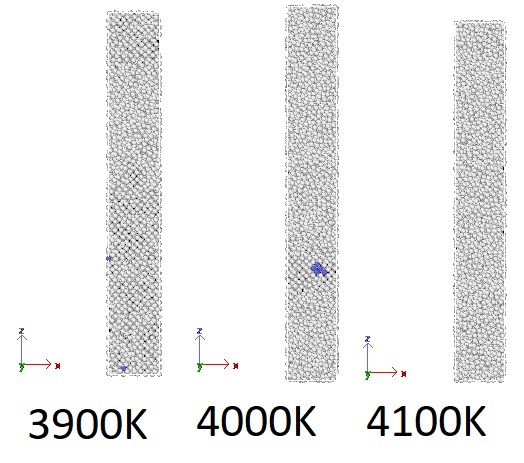
\includegraphics[width=0.7\linewidth]{inc/ovito}}
	\caption{OVITO}
	\label{ovito}
\end{figure}

По процентному содержанию кристаллов BCC видно, что плавление происходит между 4000К и 4100К.

Для уточнения проведём серию расчетов с начальными температурами от 4010К до
4090К с шагом 10 К. В этих расчетах для повышения точности увеличим
длительность в 65 строке до 45000 шагов.

На рисунке \ref{ovito2} приведено процентное содержание целых кристаллов. Можно увидеть что 0\% появляются при температуре 4030 K.

\begin{figure}[h]
	\center{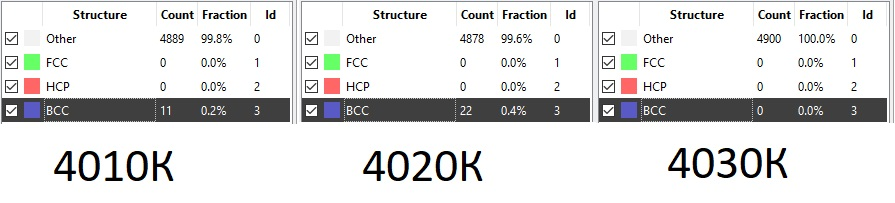
\includegraphics[width=1\linewidth]{inc/ovito2}}
	\caption{OVITO - процентное содержание кристаллов}
	\label{ovito2}
\end{figure}

\newpage
Рассмотрим ход температуры со временем при начальных значениях от 4010 до
4030 К:

\begin{figure}[!h]
	\center{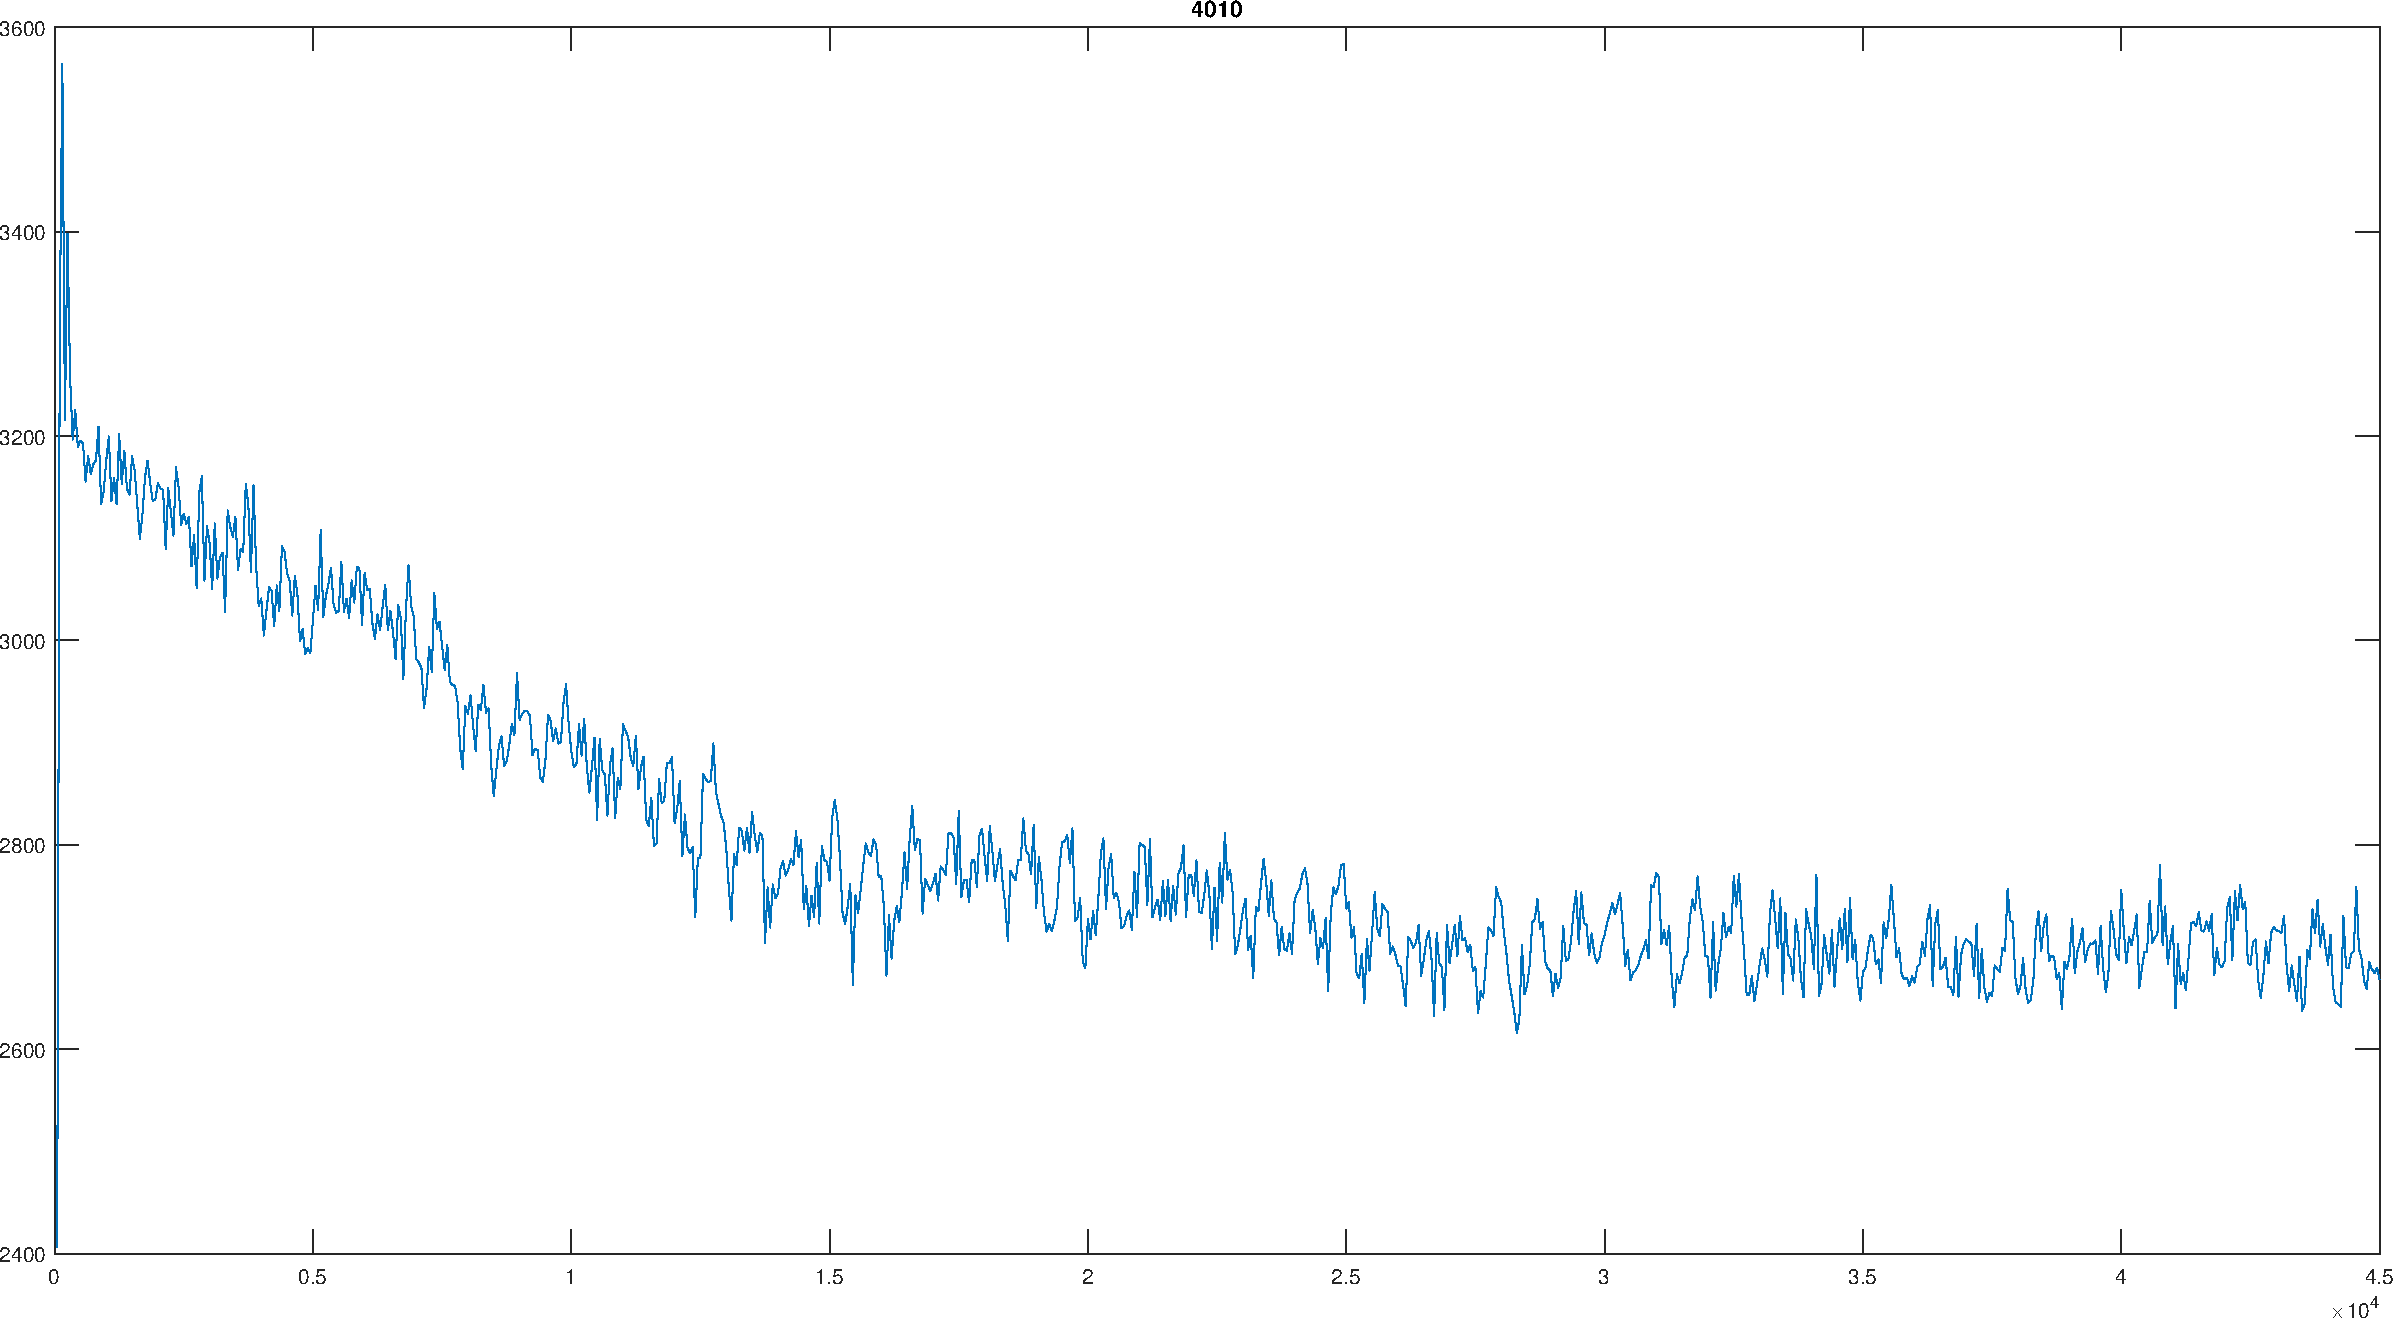
\includegraphics[width=1\linewidth]{inc/untitled1}}
	\caption{4010 K}
	\label{untitled1}
\end{figure}

%\newpage
\begin{figure}[!h]
	\center{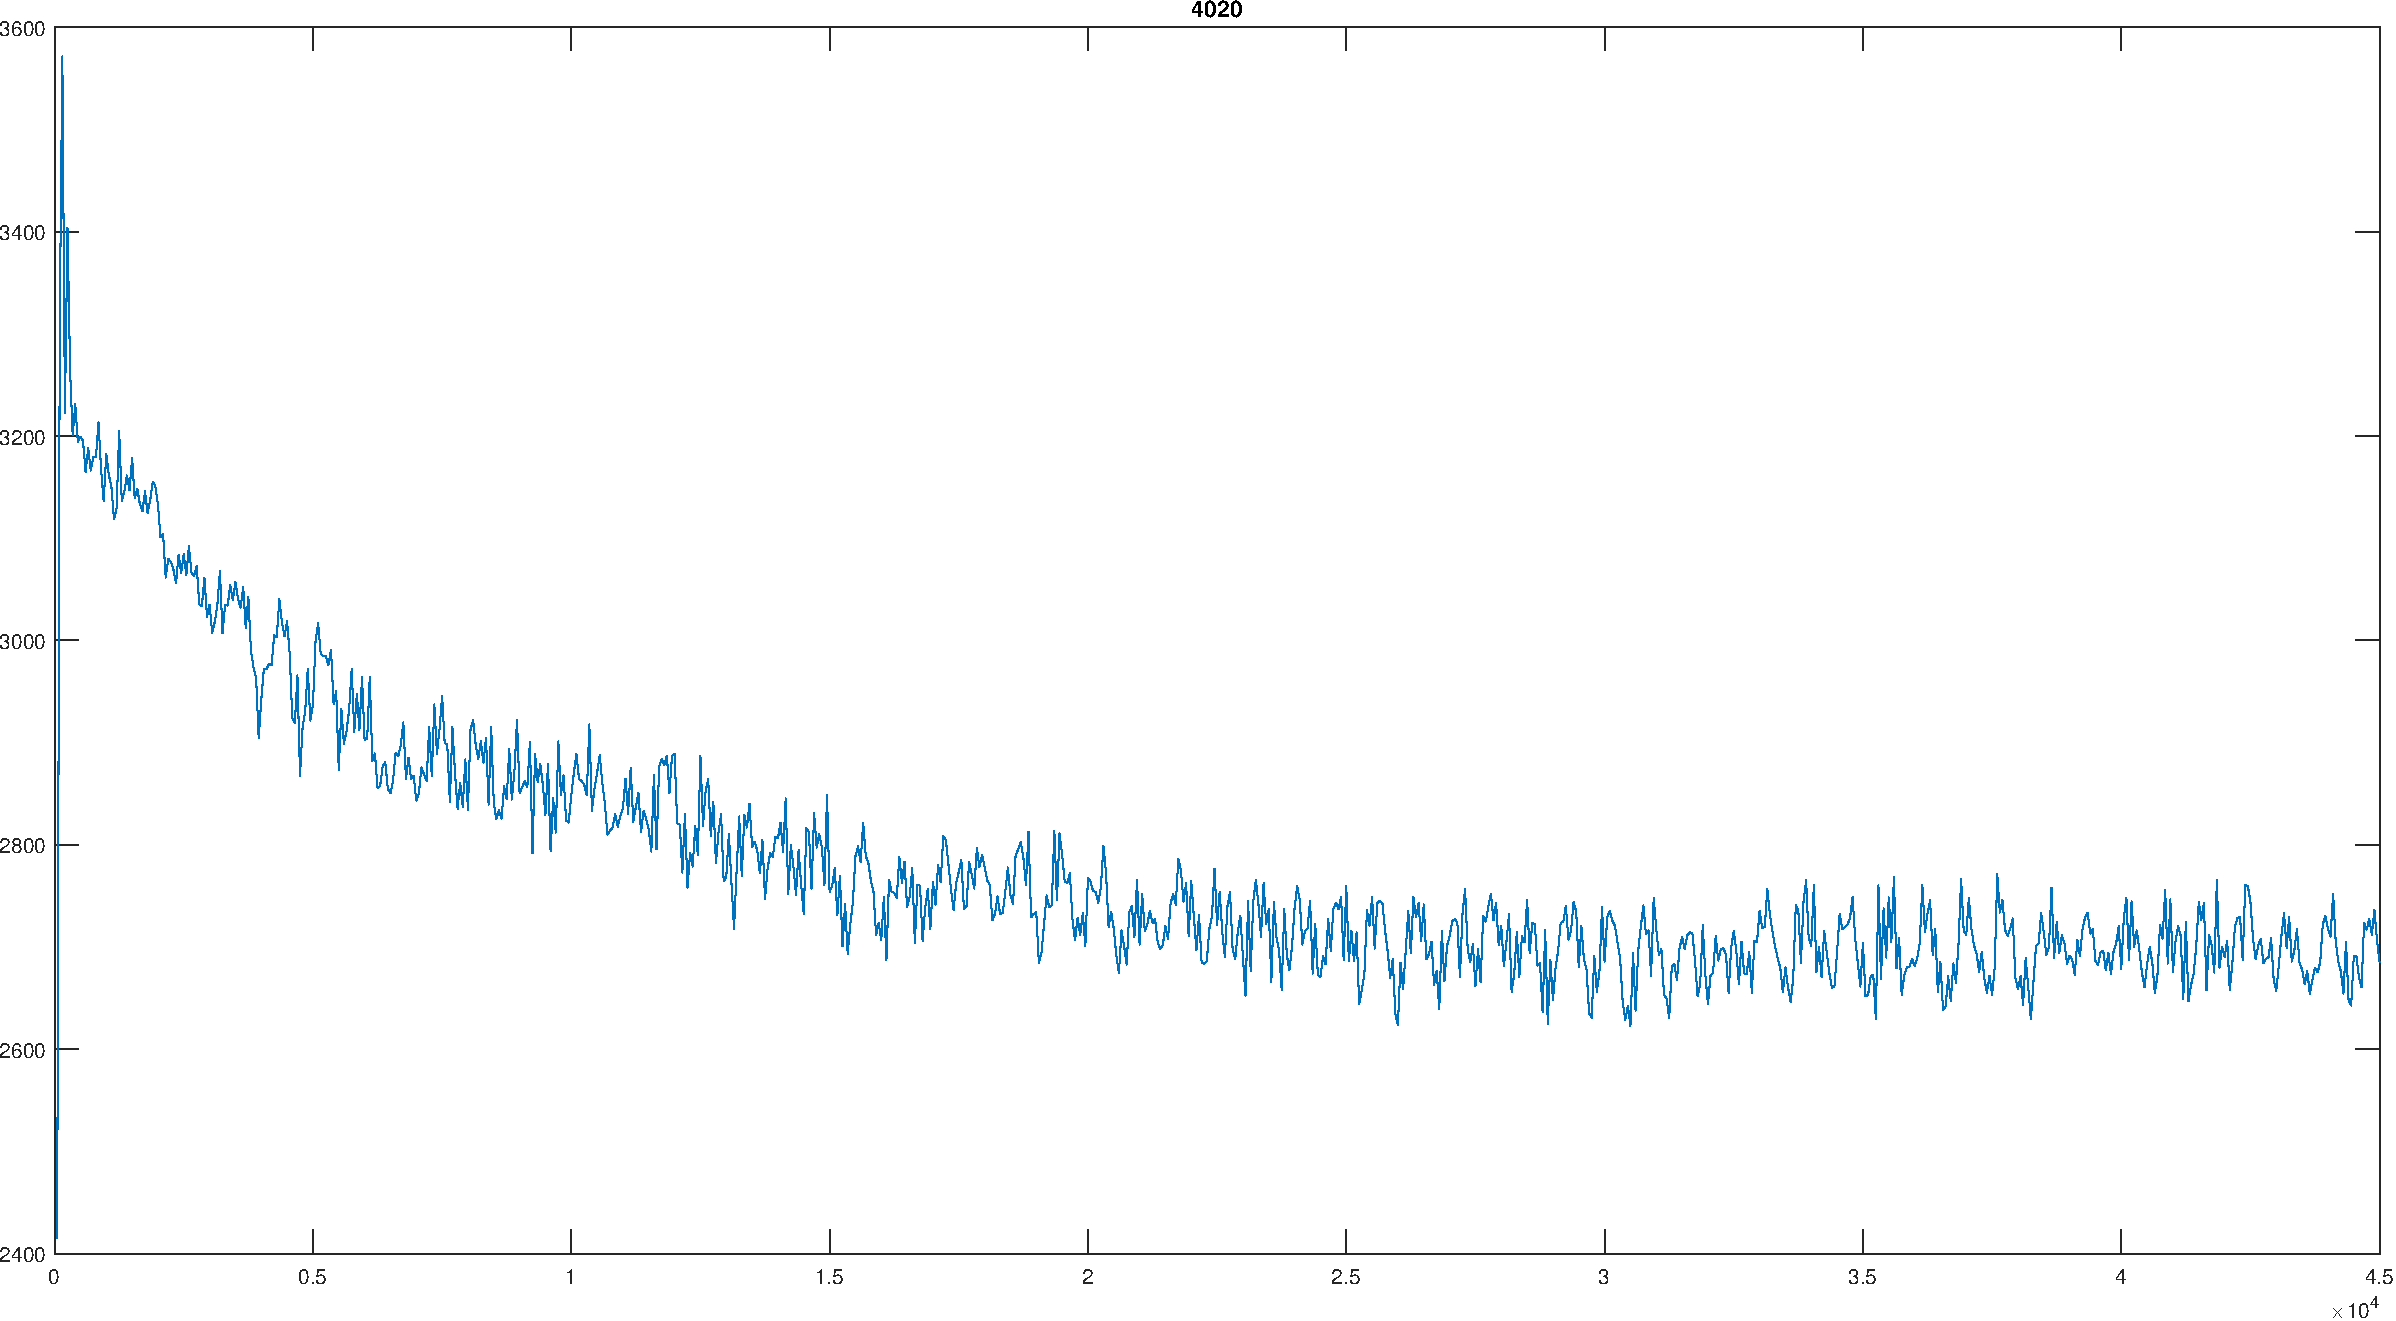
\includegraphics[width=1\linewidth]{inc/untitled2}}
	\caption{4020 K}
	\label{untitled2}
\end{figure}

\begin{figure}[!h]
	\center{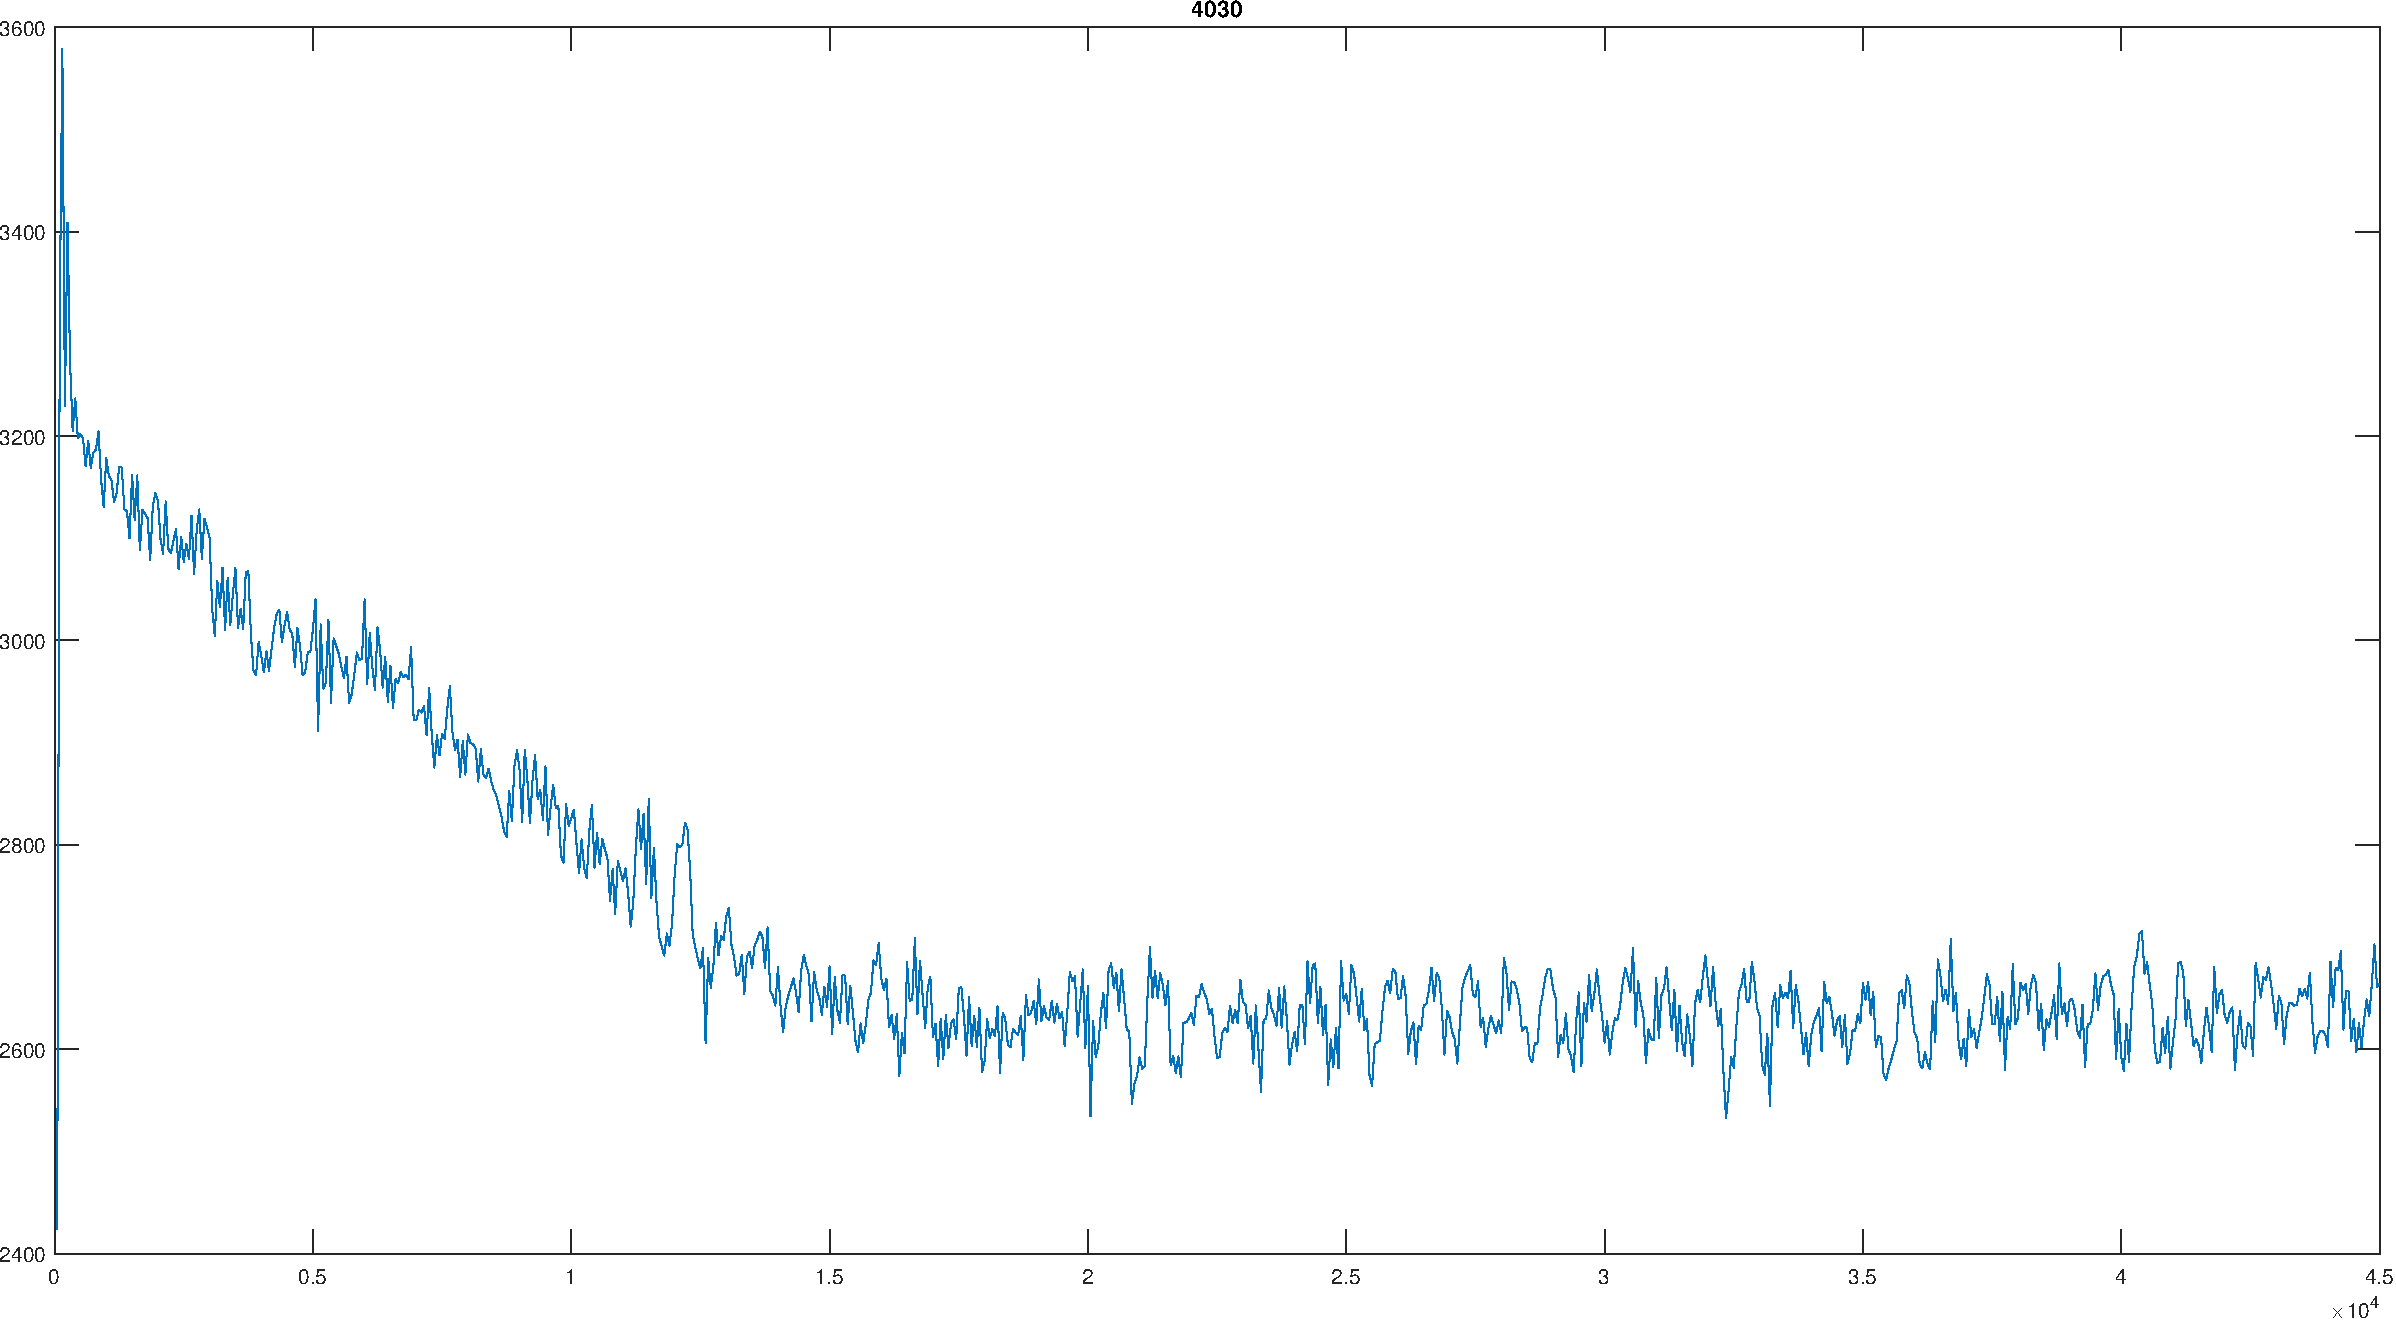
\includegraphics[width=1\linewidth]{inc/untitled3}}
	\caption{4030 K}
	\label{untitled3}
\end{figure}

\newpage
Видно, что в случае 4030 К система явно выходит к равновесию через 15000 шагов. Усредняя температуру по этому участку, получаем температуру плавления 2634 К
(табличная температура плавления 2741,15 К).

Рассмотрим графики зависимости средней температуры системы от задаваемой и от энтальпии (рис. \ref{z1}-\ref{z2}):

\begin{figure}[!h]
	\center{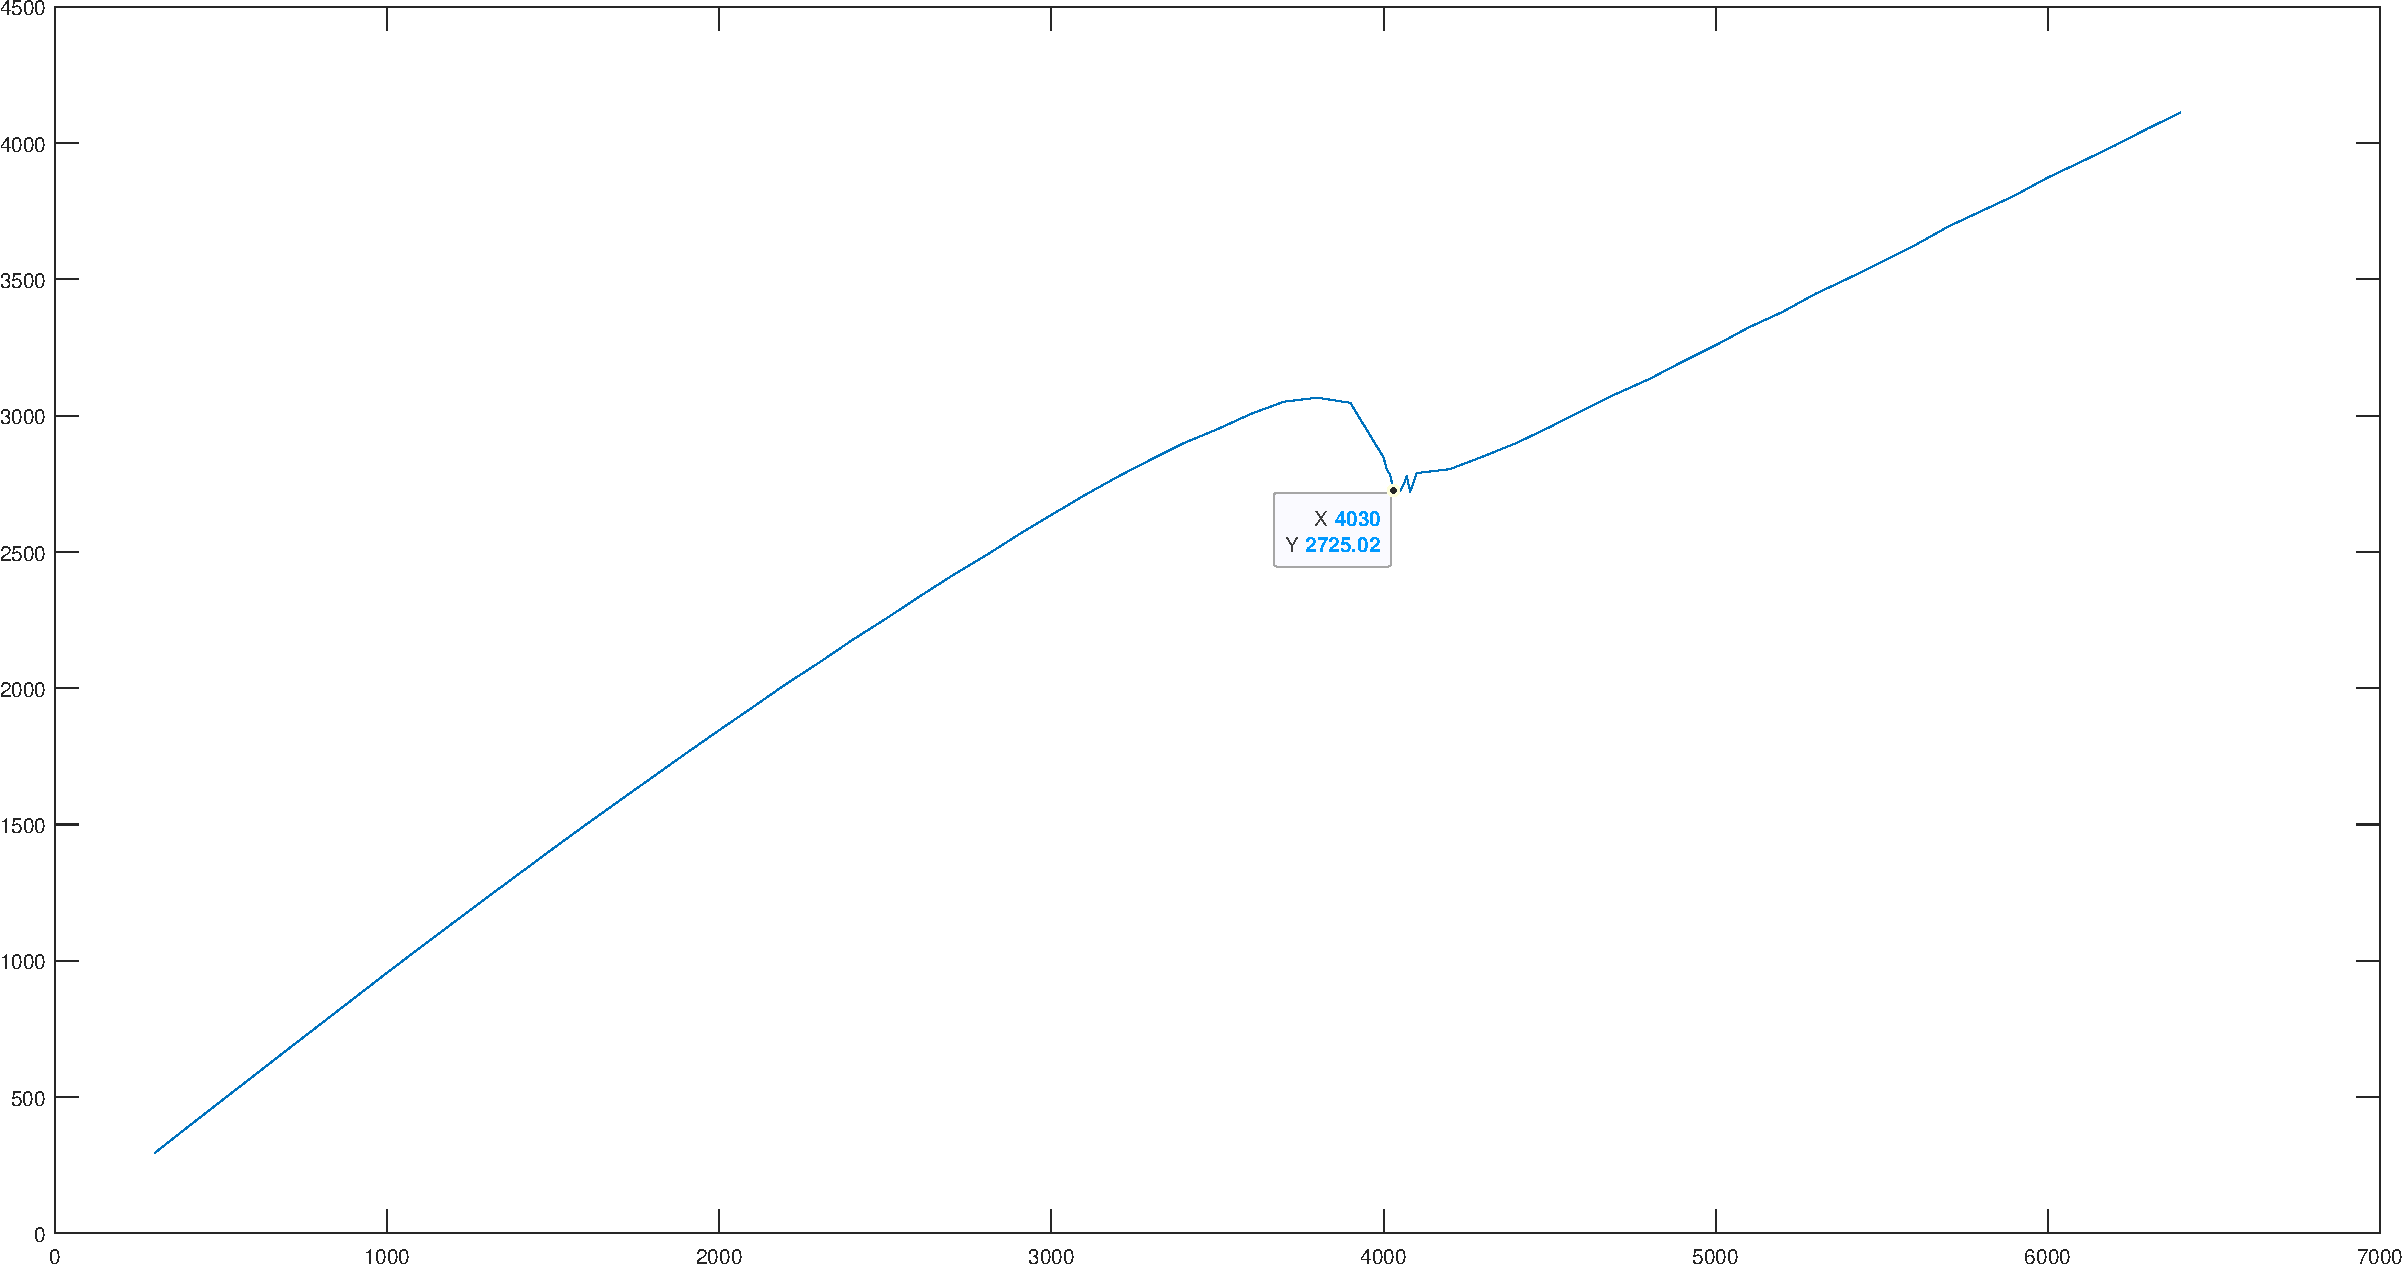
\includegraphics[width=1\linewidth]{inc/z1}}
	\caption{Зависимость средней температуры системы от задаваемой}
	\label{z1}
\end{figure}

\begin{figure}[!h]
	\center{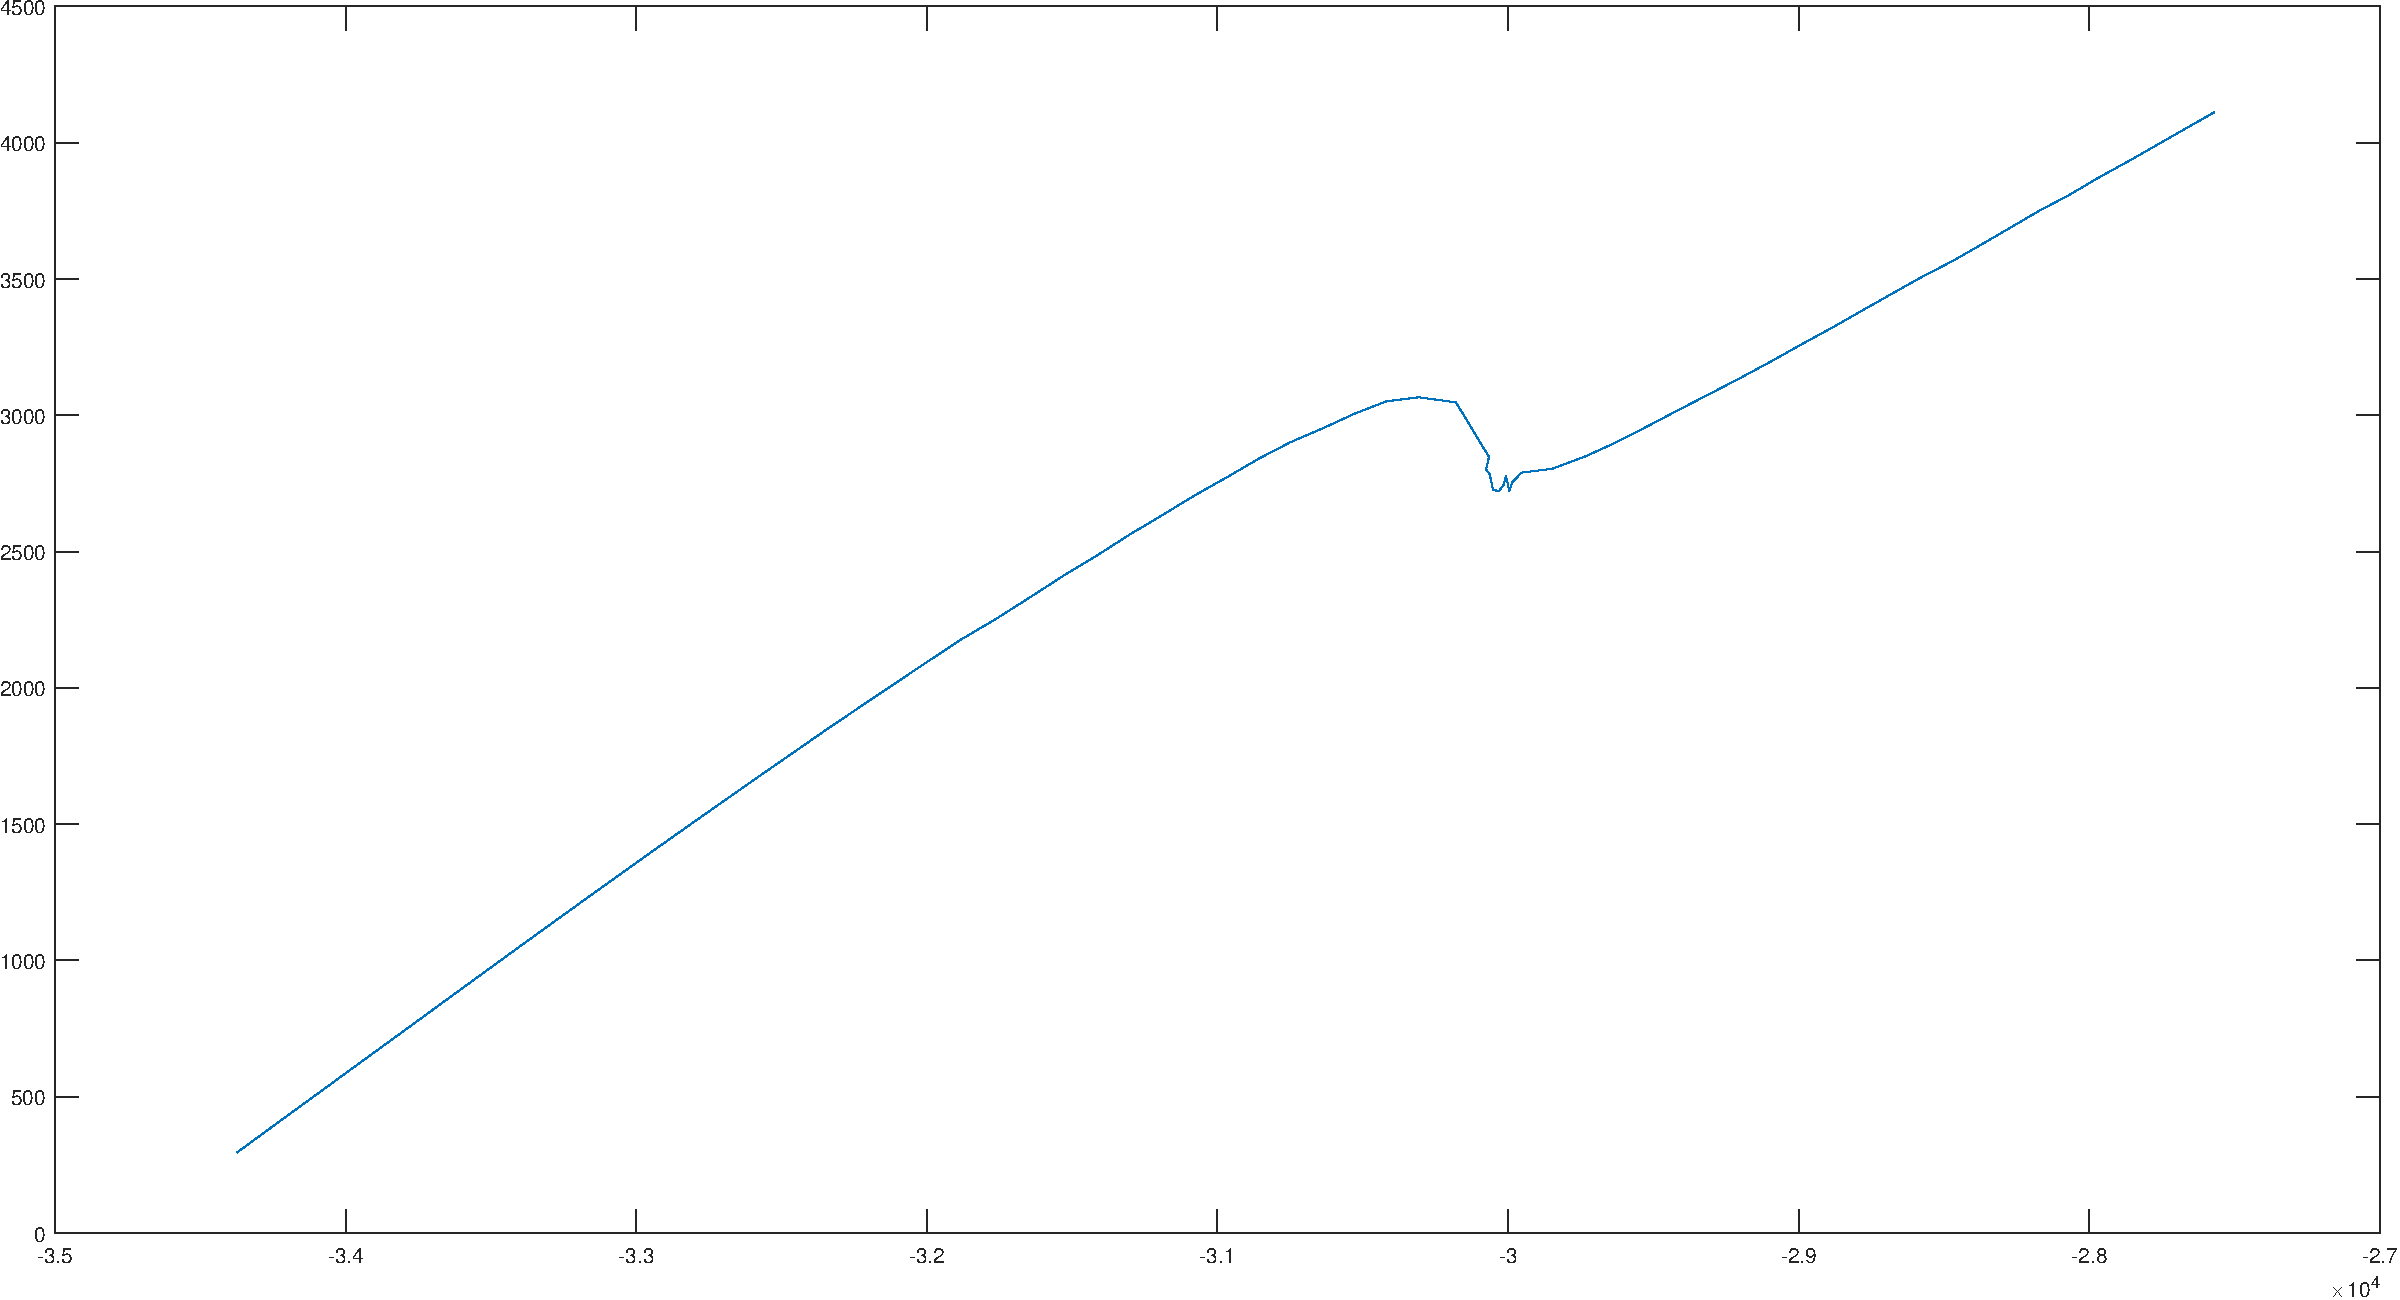
\includegraphics[width=1\linewidth]{inc/z2}}
	\caption{Зависимость средней температуры системы от энтальпии}
	\label{z2}
\end{figure}

\newpage
Как видно по -1ому графику (рис. \ref{z1}) как раз при задаваемых 4080 К получается минимальная средняя температура. А во 2-ом графике (рис. \ref{z2}) явно наблюдается провал температуры с ростом энергии, ожидаемый в Z-методе.

\newpage
\section*{Задание 2}
Запустим для температуры 2634 К расчеты с однофазным кристаллом и
жидкостью:

\textbf{lmp -in in.crystal -v lattice\_type bcc -v a0 3.3079 -v T\_init 2634 -v element\_name Nb -v atomic\_mass 92.9 -v potential\_type "eam/alloy" -v potential\_file "./Nb.eam.alloy"}

\textbf{lmp -in in.liquid -v lattice\_type bcc -v a0 3.3079 -v T\_init 2634 -v element\_name Nb -v atomic\_mass 92.9 -v potential\_type "eam/alloy" -v potential\_file "./Nb.eam.alloy"}

\begin{figure}[!h]
	\center{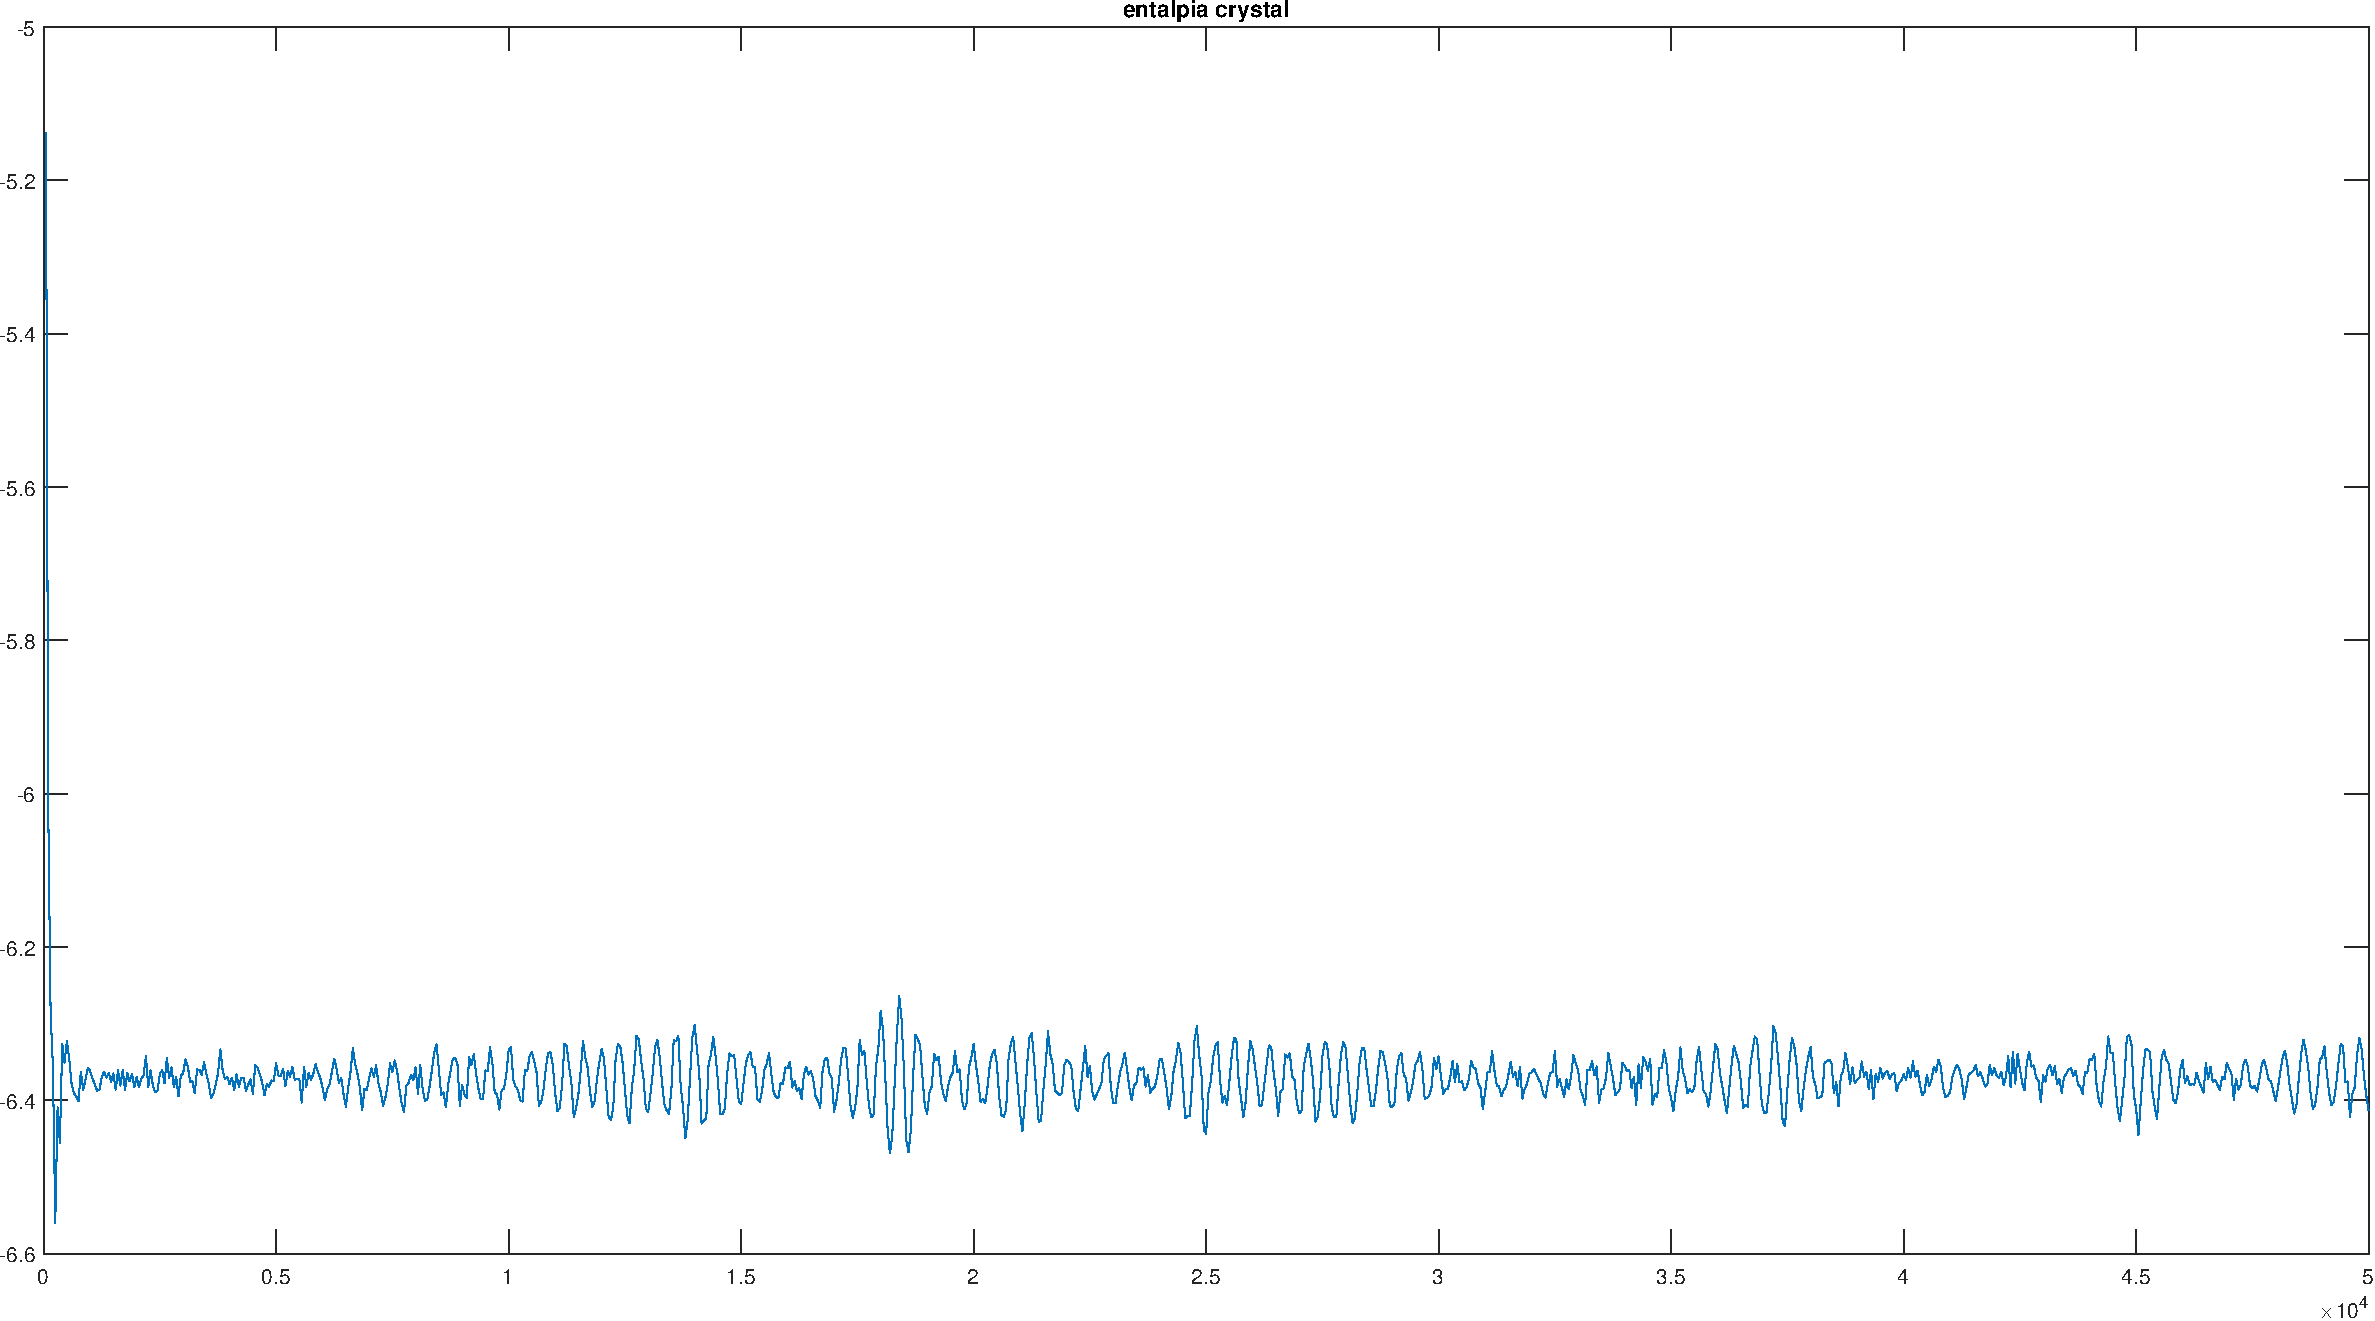
\includegraphics[width=1\linewidth]{inc/entalpia crystal}}
	\caption{entalpia crystal}
	\label{entalpia crystal}
\end{figure}

\newpage
\begin{figure}[!h]
	\center{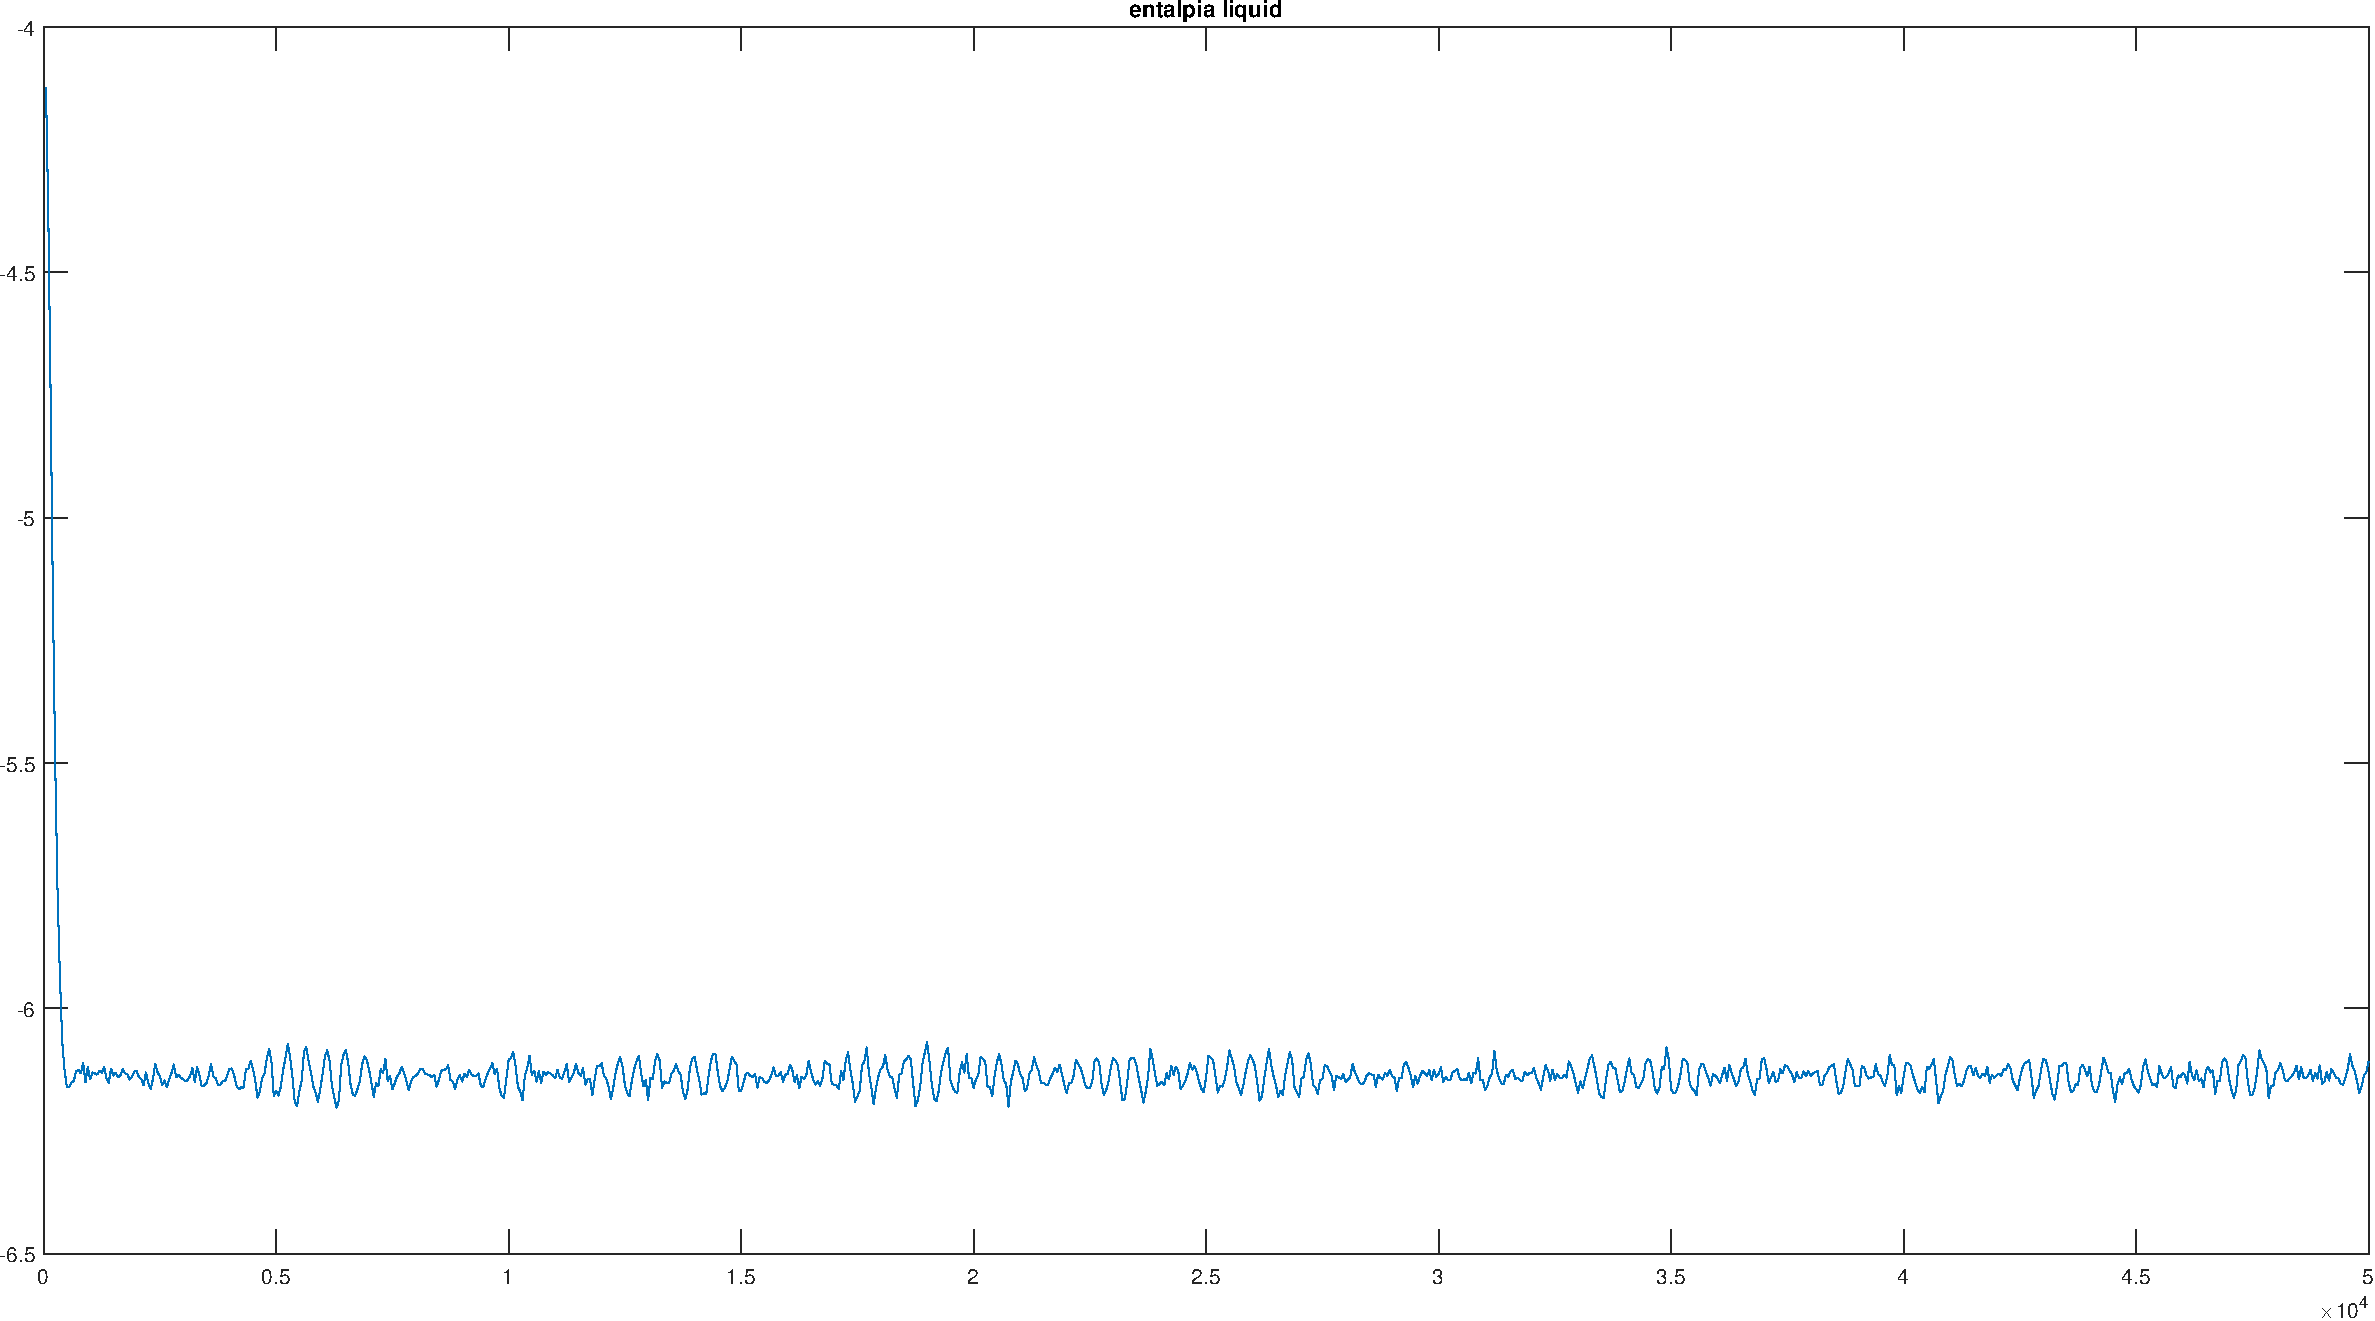
\includegraphics[width=1\linewidth]{inc/entalpia liquid}}
	\caption{entalpia liquid}
	\label{entalpia liquid}
\end{figure}

\begin{figure}[!h]
	\center{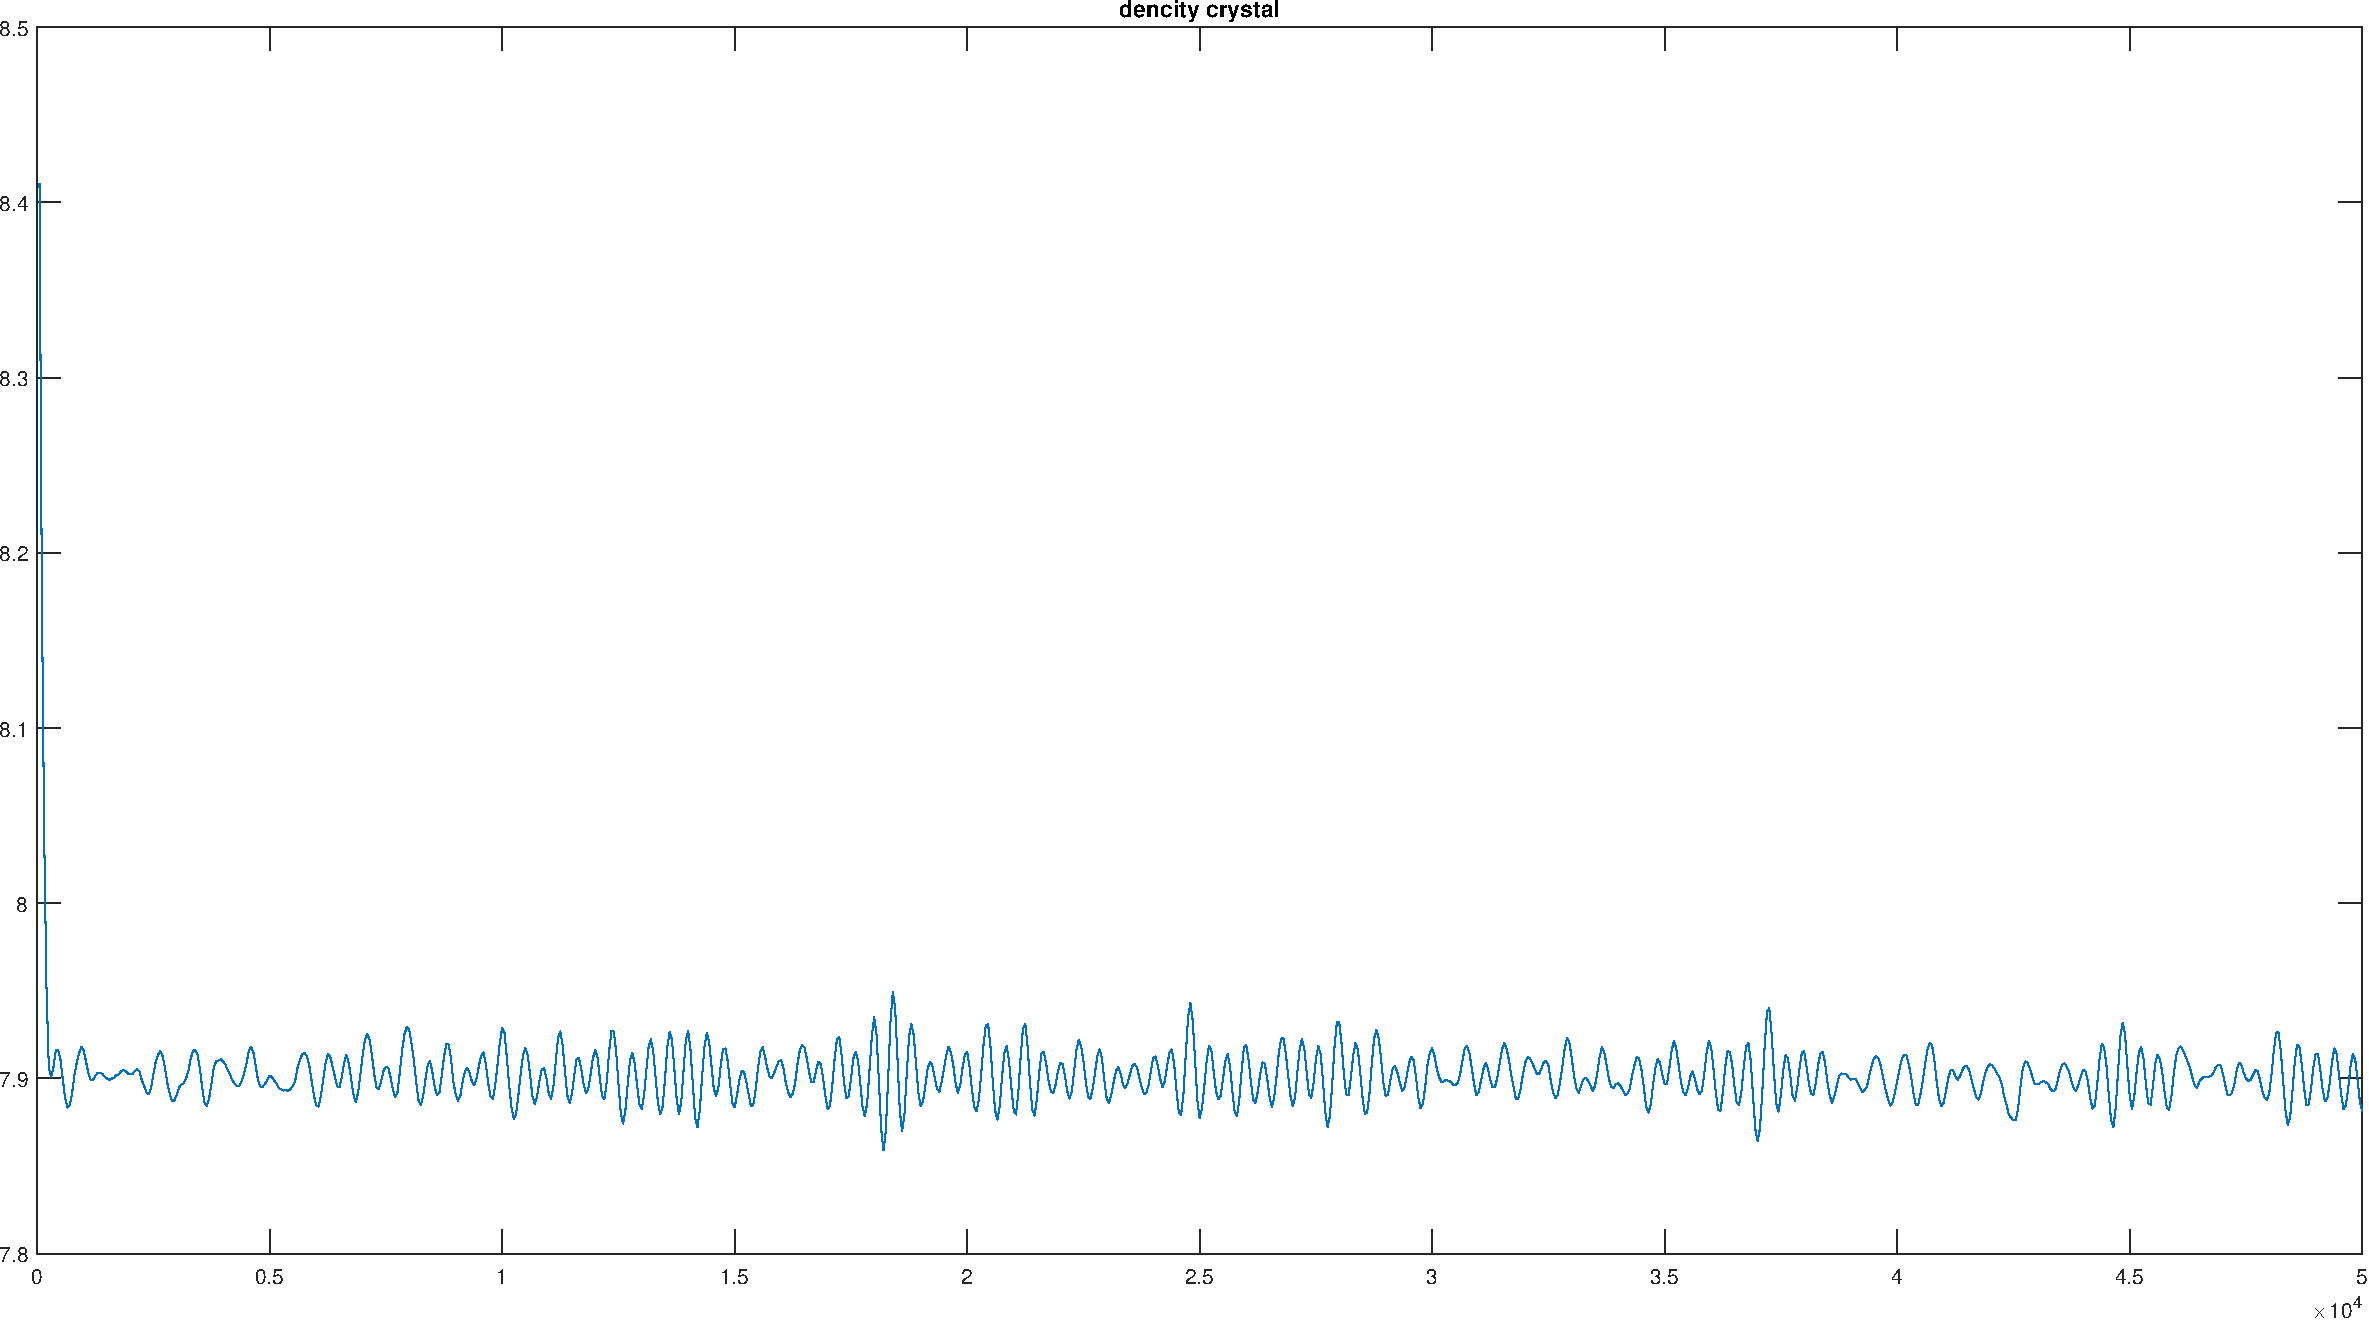
\includegraphics[width=1\linewidth]{inc/dencity crystal}}
	\caption{density crystal}
	\label{dencity crystal}
\end{figure}

\newpage
\begin{figure}[!h]
	\center{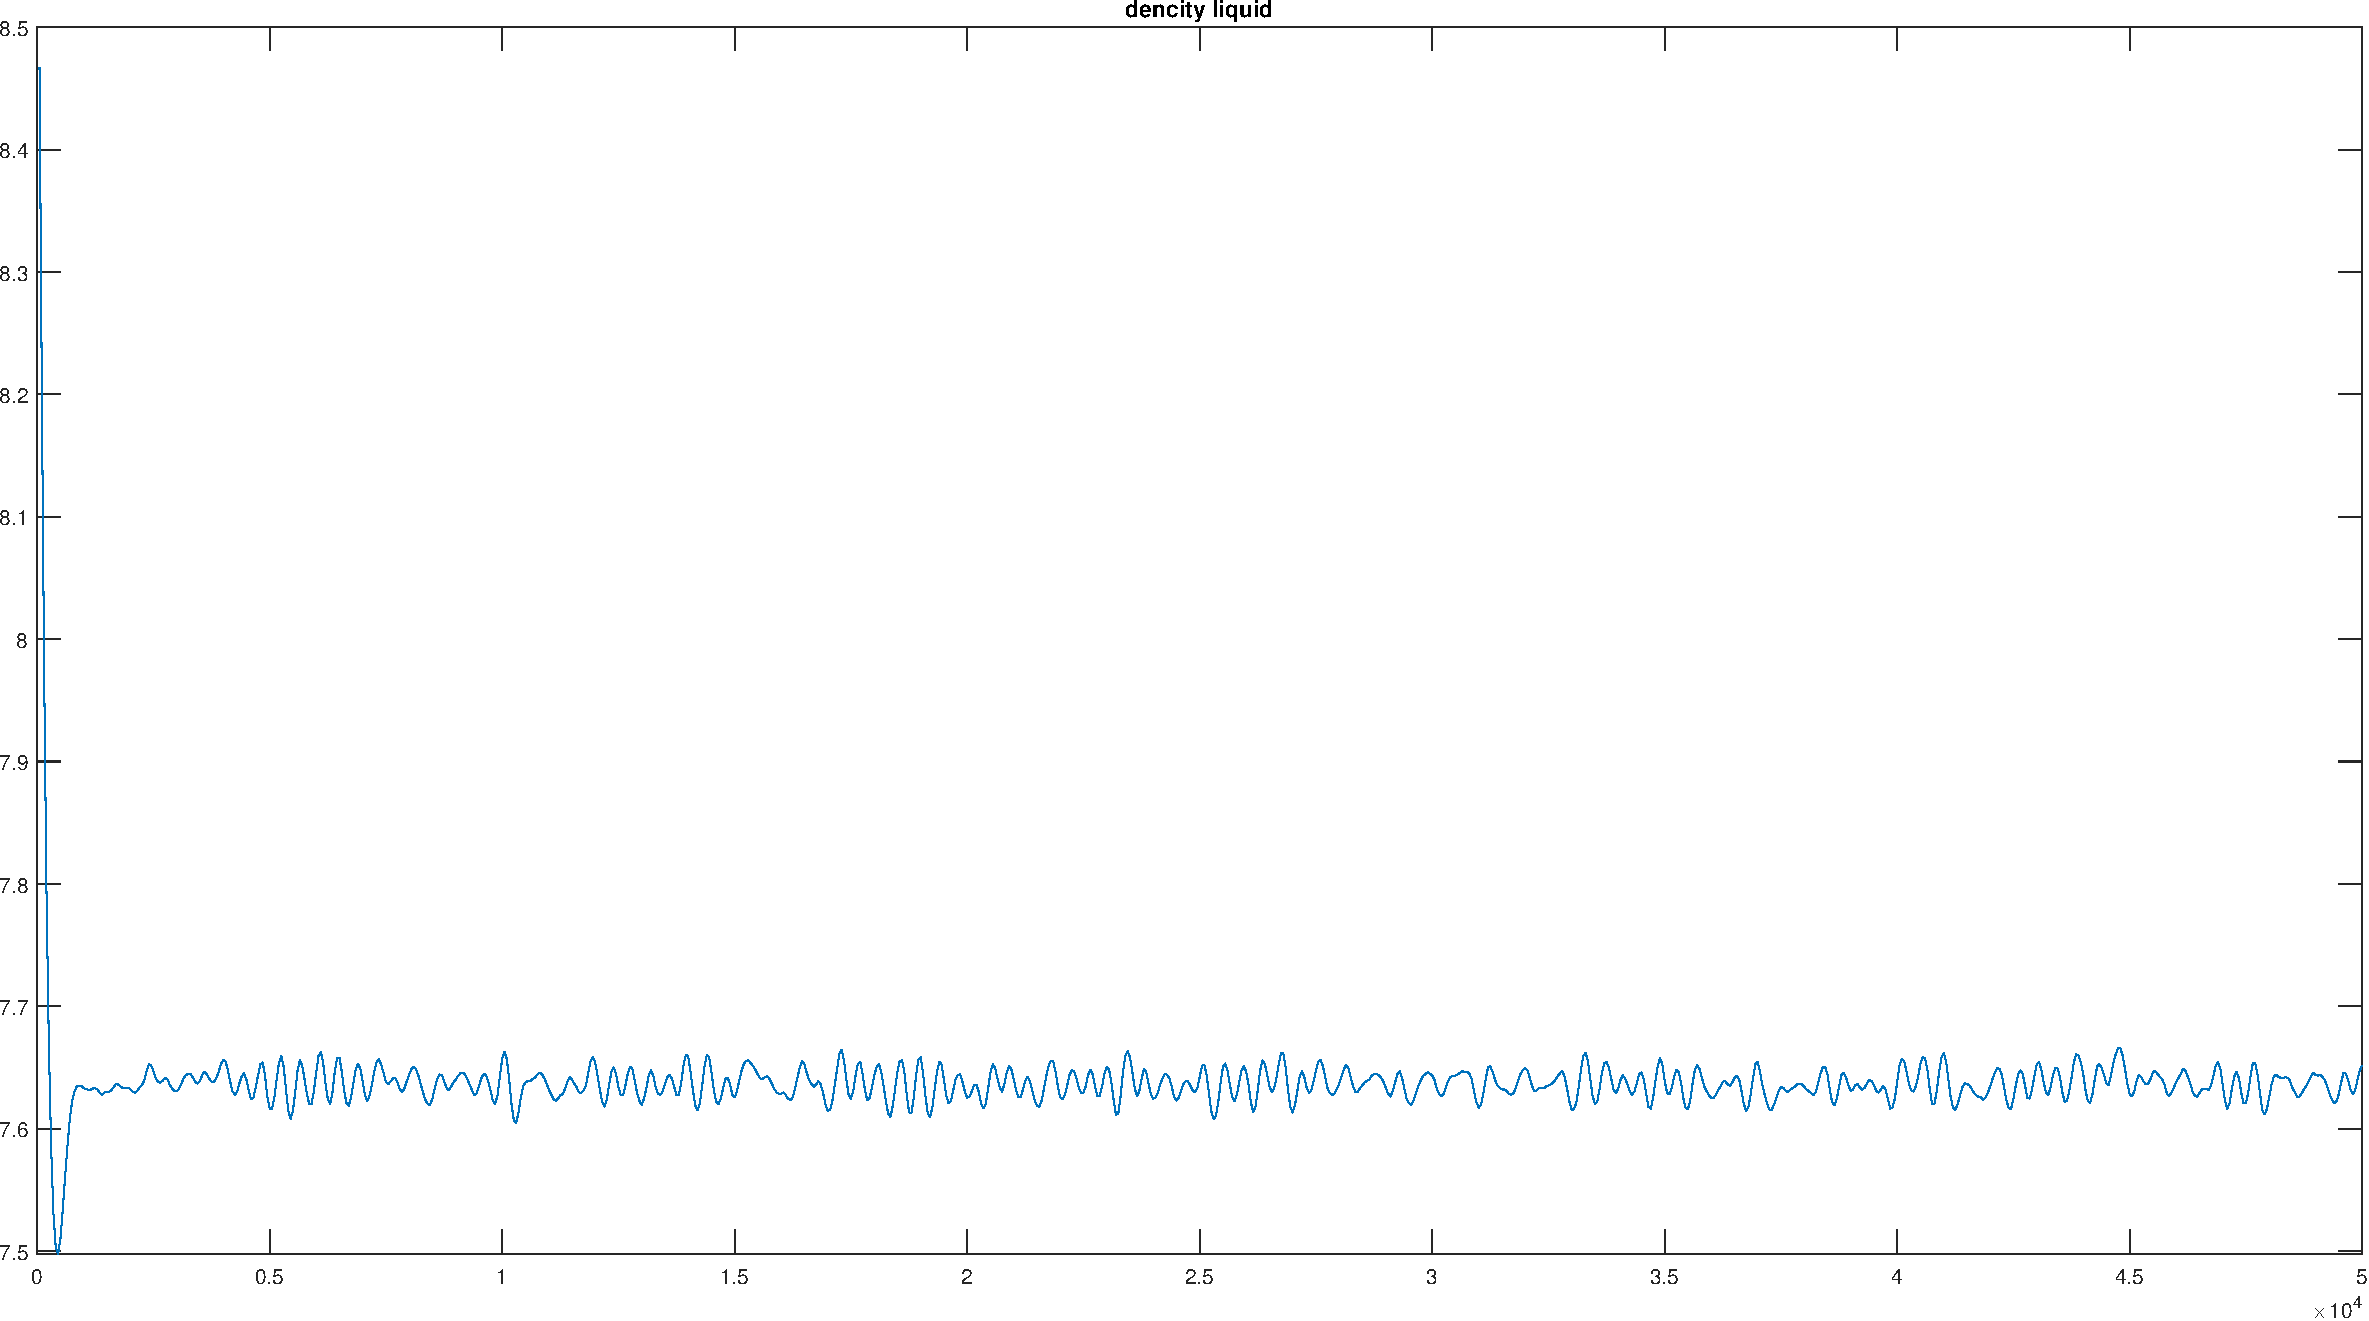
\includegraphics[width=1\linewidth]{inc/dencity liquid}}
	\caption{density liquid}
	\label{dencity liquid}
\end{figure}

После усреднения получаем плотность кристалла на линии плавления 7.9026 г/см$^3$,
плотность жидкости 7.6378 г/см$^3$. Разница плотностей 0.2649 г/см$^3$.
Энтальпия кристалла -6.3699 эВ/атом, жидкости -6.1304 эВ/атом. Теплота плавления
0.2395 эВ/атом = 23.1117 кДж/моль (табличное значение 26.4 кДж/моль).

Погрешность температуры плавления 188.4622 К, а по факту вычисленное значение температуры плавления Ниобия 2634 К отличается от табличного (2741.15 К) на 106.85 К
\end{document}